\section{Foundation Model Improvement}
\label{sec:Foundation_Model_Improvement}

% ==============algorithm pseudo-code================
\AlgoSel=3 % Algorithm 1 v3 (aligned + more inclusive, no overflow)
\ifnum\AlgoSel=3
\begin{wrapfigure}{r}{0.52\columnwidth}
\vspace{-\intextsep}
\centering

\scalebox{0.52}{%
\begin{minipage}{\columnwidth}
\begin{mdframed}[
  backgroundcolor=algobg,
  roundcorner=5pt,
  linewidth=0pt,
  innerleftmargin=4pt,
  innerrightmargin=4pt,
  innertopmargin=4pt,
  innerbottommargin=4pt
]
\begingroup
\SetAlFnt{\large}   
\SetAlCapFnt{\large}  
\SetAlCapNameFnt{\large} 
\begin{algorithm}[H]
\caption{Foundation\mbox{-}Model Improvement}
\label{alg:foundation_model_improvement}

\SetKwInOut{Input}{Input}
\SetKwInOut{Output}{Output}
\Input{Initial agent state $\mathcal{A}_0=(\theta_0,\Sigma)$; maximum iterations $T$}
\Output{Improved agent $\mathcal{A}_T=(\theta_T,\Sigma)$}

\BlankLine
\For{$t \leftarrow 0$ \KwTo $T-1$}{

  \textcolor{RoyalBlue}{\tcp{1) Construct or collect learning signal $\mathcal{S}_t$}}
  $\mathcal{S}_t \leftarrow \emptyset$

  \If{subcategory includes intrinsic generative demonstrations}{%
    $\mathcal{S}_t \leftarrow \mathcal{S}_t \cup \textsc{GenerateDemonstrations}(\mathcal{A}_t)$
    \tcp*{\S \ref{sec:Intrinsic_Generative_Demonstrations}}
  }
  \If{subcategory includes intrinsic evaluative feedback}{%
    $\mathcal{S}_t \leftarrow \mathcal{S}_t \cup \textsc{GenerateEvaluativeFeedback}(\mathcal{A}_t)$
    \tcp*{\S \ref{sec:Intrinsic_Evaluative_Feedback}}
  }
  \If{subcategory includes extrinsic exploratory experience}{%
    $\mathcal{S}_t \leftarrow \mathcal{S}_t \cup \textsc{CollectExperience}(\mathcal{A}_t,\text{env})$
    \tcp*{\S \ref{sec:Extrinsic_Exploratory_Experience}}
  }

  \textcolor{gray}{\tcp{Optional: quality control / weighting of signals}}
  $\mathcal{S}_t \leftarrow \textsc{FilterOrWeight}(\mathcal{S}_t)$

  \textcolor{RoyalBlue}{\tcp{2) Parameter update}}
  $\theta_{t+1} \leftarrow \textsc{Update}(\theta_{1:t},\mathcal{S}_t)$

  \textcolor{RoyalBlue}{\tcp{3) State update}}
  $\mathcal{A}_{t+1} \leftarrow (\theta_{t+1},\Sigma)$

  \If{\textsc{Converged}($\mathcal{A}_{t+1}$)}{break}
}
\Return{$\mathcal{A}_T$}
\end{algorithm}
\endgroup
\end{mdframed}
\end{minipage}%
}

\vspace{-10pt}
\end{wrapfigure}
\fi


% Algorithm 2 v3 (aligned + more inclusive, no overflow)
\ifnum\AlgoSel=4
\begin{wrapfigure}{r}{0.52\columnwidth}
\vspace{-\intextsep}
\centering

\scalebox{0.52}{%
\begin{minipage}{\columnwidth}
\begin{mdframed}[
  backgroundcolor=algobg,
  roundcorner=5pt,
  linewidth=0pt,
  innerleftmargin=4pt,
  innerrightmargin=4pt,
  innertopmargin=4pt,
  innerbottommargin=4pt
]
\begingroup
\SetAlFnt{\large}   
\SetAlCapFnt{\large}  
\SetAlCapNameFnt{\large} 
\begin{algorithm}[H]
\caption{Scaffolding Improvement}
\label{alg:scaffolding_improvement}

\SetKwInOut{Input}{Input}
\SetKwInOut{Output}{Output}
\Input{Initial agent state $\mathcal{A}_0=(\theta,\Sigma_0)$; max iterations $T$}
\Output{Improved agent $\mathcal{A}_T=(\theta,\Sigma_T)$}

\BlankLine
\For{$t \leftarrow 0$ \KwTo $T-1$}{

  \textcolor{RoyalBlue}{\tcp{1) Collect scaffolding learning signal $\mathcal{S}_t$}}
  $\mathcal{S}_t \leftarrow \textsc{InteractAndEvaluate}(\mathcal{A}_t,\text{env})$
  \tcp*{\footnotesize traces, critiques, success/failure, cost}

  \textcolor{gray}{\tcp{Optional: quality control / weighting of signals}}
  $\mathcal{S}_t \leftarrow \textsc{FilterOrWeight}(\mathcal{S}_t)$

  \textcolor{RoyalBlue}{\tcp{2) Scaffolding update (keep $\theta$ fixed)}}
  \uIf{subcategory = Full scaffolding}{%
    $\Sigma_{t+1} \leftarrow \IMPROVE_{\Sigma}(\Sigma_{1:t};\mathcal{S}_t)$
    \tcp*{\S~\ref{sec:Full_Scaffolding}}
  }
  \Else{%
    $p_{t+1} \leftarrow p_t$; $m_{t+1} \leftarrow m_t$; $\mathcal{T}_{t+1} \leftarrow \mathcal{T}_t$

    \If{subcategory includes Prompt-based}{%
      $p_{t+1} \leftarrow \IMPROVE_{p}(p_t;\mathcal{S}_t)$
      \tcp*{\S~\ref{sec:Prompt_Optimization}}
    }
    \If{subcategory includes Memory-based}{%
      $m_{t+1} \leftarrow \IMPROVE_{m}(m_t;\mathcal{S}_t)$
      \tcp*{\S~\ref{sec:Memory}}
    }
    \If{subcategory includes Tool-based}{%
      $\mathcal{T}_{t+1} \leftarrow \IMPROVE_{\mathcal{T}}(\mathcal{T}_t;\mathcal{S}_t)$
      \tcp*{\S~\ref{sec:Tool}}
    }

    $\Sigma_{t+1} \leftarrow (p_{t+1},\, m_{t+1},\, \mathcal{T}_{t+1})$
  }

  \textcolor{RoyalBlue}{\tcp{3) State update}}
  $\mathcal{A}_{t+1} \leftarrow (\theta,\Sigma_{t+1})$
}
\Return{$\mathcal{A}_T$}
\end{algorithm}
\endgroup
\end{mdframed}
\end{minipage}%
}

\vspace{-16pt}
\end{wrapfigure}
\fi
% ==============algorithm pseudo-code================

Foundation-model-based self-improvement constitutes one of the most direct pathways for enhancing an agent’s intrinsic capabilities. This approach targets the agent’s core, namely the parameter set $\theta_{t}$ of its underlying FM, and updates these parameters to internalize new behaviors and reasoning patterns~\citep{wang2022self, bai2022constitutional, shafayat2025can, bensal2025reflect, dong2025tool, wang2025ragenunderstandingselfevolutionllm, zhou2025selfchallenging}. Such updates are typically achieved through gradient-based optimization, resulting in stable changes to the model weights. In this sense, the FM is treated as a continually learnable system that stores improvements in its parametric memory, rather than relying solely on transient execution states. Because the model parameters compress the agent's learned representations and behavioral priors, updating them allows the agent to fundamentally refine its policy, reduce systematic errors, and improve alignment with target objectives. In practice, the agent effectively serves as its own source of supervision: it uses its own execution to generate training signals—such as demonstrations, evaluations, or interaction trajectories—and applies learning algorithms to these self-induced signals to systematically improve its capabilities over successive updates.

To systematically analyze FM-based self-improvement, we classify existing methods by the nature of how the learning signal $\mathcal{S}_t$ is used to update the foundation-model parameters under our formalism. Consistent with the history-aware operator in Section~\ref{sec:Definitions}, we write the transition as $\mathcal{A}_{t+1}=\text{IMPROVE}(\mathcal{A}_{1:t};\mathcal{S}_t)$ with $\theta_{t+1}=\text{IMPROVE}_{\theta}(\theta_{1:t};\mathcal{S}_t)$ and $\Sigma_{t+1}=\Sigma_t$, allowing validation and rollback to prior checkpoints when necessary. This taxonomy yields three principal subcategories:
(i) \textbf{Intrinsic generative demonstrations} (\S \ref{sec:Intrinsic_Generative_Demonstrations}), where the learning signal is instantiated as $\mathcal{S}_t \approx \mathcal{D}_t$: the FM-based agent generates explicit examples, demonstrations, or task--solution pairs that are used for parameter updates.
(ii) \textbf{Intrinsic evaluative feedback} (\S \ref{sec:Intrinsic_Evaluative_Feedback}), where the learning signal is instantiated as $\mathcal{S}_t \approx e_t$: the FM-based agent or an internal evaluator judges candidate behavior through scores, preferences, confidence estimates, consistency signals, critiques, or revisions, which are then used to update the foundation model.
(iii) \textbf{Extrinsic exploratory experience} (\S \ref{sec:Extrinsic_Exploratory_Experience}), where the learning signal is instantiated as $\mathcal{S}_t \approx \tau_t$: the agent collects trajectories, rewards, observations, or executable outcomes through interaction with external or simulated environments. These subcategories are not mutually exclusive in deployed systems. Many practical pipelines mix intrinsic demonstrations, intrinsic evaluations, and exploratory experience within a single improvement cycle; for clarity, we categorize methods by the dominant signal source and objective used in their update operator. Algorithm~\ref{alg:foundation_model_improvement} summarizes the generic update loop of foundation-model improvement under self-generated learning signals.


% ==============figure-5-1================
\begin{figure*}[ht]
    \centering
    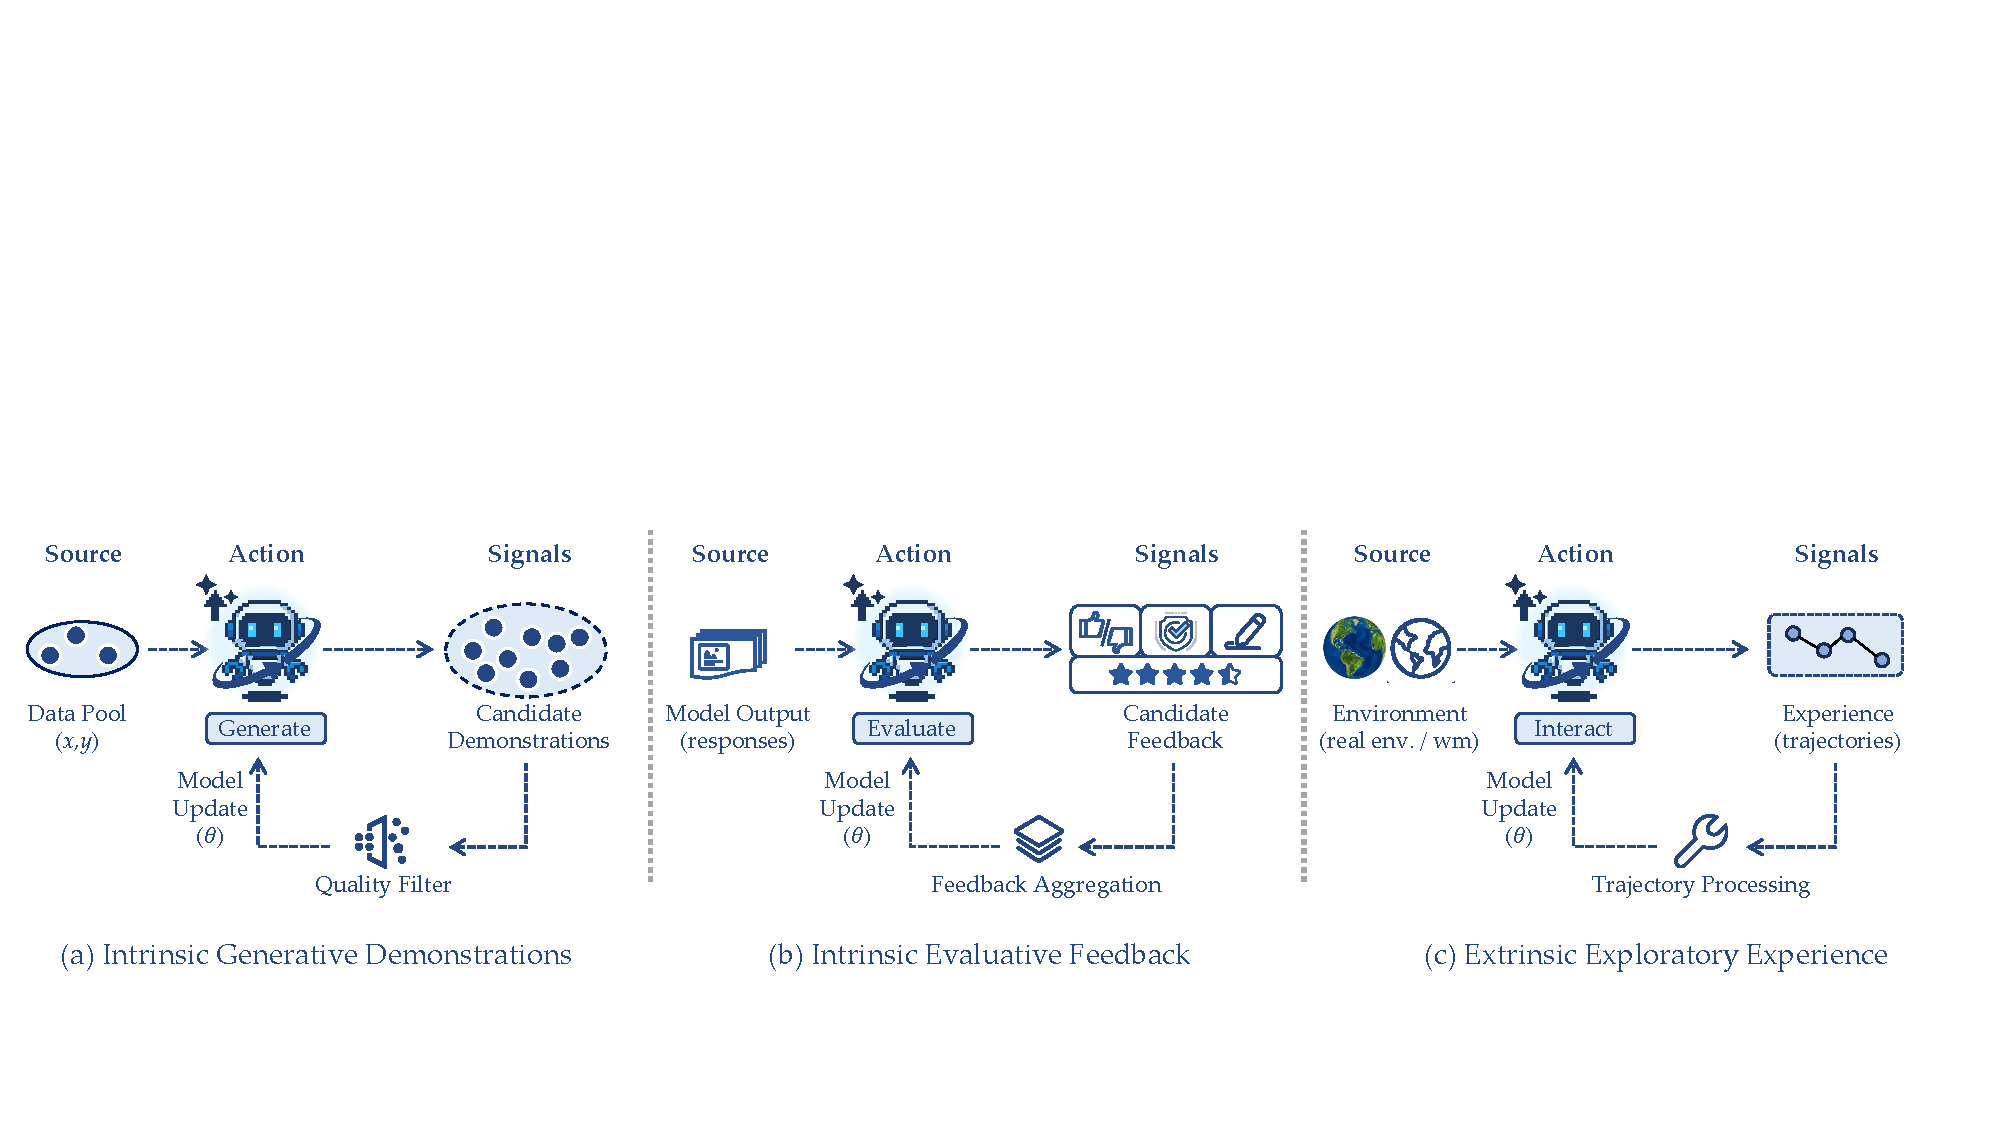
\includegraphics[width=\linewidth]{fig/fig-FMI.pdf}
    \caption{Overview of foundation model improvement under agent-induced learning signals. The agent improves the foundation model by generating intrinsic demonstrations, producing intrinsic evaluative feedback, or collecting extrinsic exploratory experience, each forming a distinct parameter-update loop.}
    \label{fig:FMI}
\end{figure*}
% ==============figure-5-1================


\subsection{Intrinsic Generative Demonstrations}
\label{sec:Intrinsic_Generative_Demonstrations}
\label{sec:Self_Generated_Data}

The remarkable capabilities of modern foundation models are fundamentally driven by their massive parameter scales, which inherently demand vast quantities of high-quality training data to continuously optimize and align~\citep{zhao2024selfguidebettertaskspecificinstruction, gan2025theoreticalunderstandingsyntheticdata}. The methods in this category fall into the group of internal generative processes, where FMs act simultaneously as the cognitive learner and the data synthesizer~\citep{zhao2024selfguidebettertaskspecificinstruction, zweiger2025selfadapting}. Leveraging the  semantic priors already compressed within their weights, FM-based agents can autonomously construct intrinsic generative demonstrations in forms such as instruction-response pairs, reasoning trajectories, and execution logs, without requiring new external observations~\citep{zhao2024selfguidebettertaskspecificinstruction, shi2025taskcraft, simonds2025ladder}. By casting the agent as its own data provider, this paradigm shifts the bottleneck of parameter updates from the costly acquisition of human annotations to the design of effective generation strategies and internal filtering mechanisms~\citep{qin2025dive}. 

Formally, as illustrated in Fig. \ref{fig:FMI} (a), under foundation-model improvement we treat these intrinsic generative demonstrations as the learning signal, i.e., $\mathcal{S}_t \approx \mathcal{D}_t$. At iteration $t$, the agent state $\mathcal{A}_t=(\theta_t,\Sigma_t)$ induces a generative distribution $\mathcal{P}_{\mathrm{gen}}(x,y \mid \mathcal{A}_t)$ and samples an intrinsic dataset
\begin{equation}
\mathcal{D}^{\mathrm{gen}}_t=\{(x_i,y_i)\}_{i=1}^{n_t}\sim \mathcal{P}_{\mathrm{gen}}(\cdot\mid \mathcal{A}_t).
\end{equation}
Optionally, a quality-control operator $\Phi_t$ filters or weights examples~\citep{jiang2025importance} to yield
$\tilde{\mathcal{D}}^{\mathrm{gen}}_t=\Phi_t(\mathcal{D}^{\mathrm{gen}}_t)$. The effective training set (and hence the learning signal) is then
$\mathcal{D}_t=\mathcal{D}^{\mathrm{base}}_t\cup \tilde{\mathcal{D}}^{\mathrm{gen}}_t$,
where $\mathcal{D}^{\mathrm{base}}_t$ denotes any existing data.


The parameter update can be written compactly as $\theta_{t+1}=\IMPROVE_{\theta}(\theta_{1:t};\mathcal{D}_t)$, where $\IMPROVE_{\theta}$ denotes the outcome of optimizing an empirical objective on $\mathcal{D}_t$ (typically initialized at the current active checkpoint $\theta_t$). We write this objective as $\mathcal{L}(\theta;\mathcal{D}_t)$, with $\Omega(\theta,\theta_0)$ an optional regularizer around an initialization $\theta_0$ and $\lambda\ge 0$ its coefficient:
\begin{equation}
\theta_{t+1}=\arg\min_{\theta}\;\mathcal{L}(\theta;\mathcal{D}_t)+\lambda\,\Omega(\theta,\theta_0).
\end{equation}
In practice, $\IMPROVE_{\theta}$ is implemented via iterative fine-tuning with a gradient-based optimizer. Let $\theta_t^{(0)}=\theta_t$, and let $\mathcal{B}_t^{(k)}$ denote a minibatch drawn from $\mathcal{D}_t$ according to the weighting induced by $\Phi_t$. Using step size $\eta_k$ at inner step $k$ and the gradient operator $\nabla_{\theta}$ with respect to $\theta$, for $k=0,\dots,K_t-1$,
\begin{equation}
\theta_t^{(k+1)}=\theta_t^{(k)}-\eta_k\,\nabla_{\theta}\mathcal{L}\big(\theta_t^{(k)};\mathcal{B}_t^{(k)}\big),
\end{equation}
and the outer-loop update is $\theta_{t+1}=\theta_t^{(K_t)}$. To systematically explore this approach, we consider three key aspects: the strategy used to generate these intrinsic demonstrations, the format of the generated data, and the challenges that arise in closing the self-improvement loop.


\paragraph{\textcolor{Plum}{Generation strategies.}}
The strategy of data generation is a critical factor for the quality and scalability of a self-improvement loop. 
% Foundational techniques bootstrap from a small seed set of examples to synthesize a larger corpus of instruction–output pairs. Moving beyond mere volume expansion, methods like Evol-Instruct \citep{xu2024wizardlm} drive {complexity evolution} by utilizing the LLM to rewrite and progressively elevate the difficulty of instructions, thereby overcoming human limitations in crafting highly complex scenarios. 
The underlying techniques start with a small set of example seeds and then build a larger instruction-output pair corpus.\citep{wang2022self, zhao2024selfguidebettertaskspecificinstruction}. Methods such as Evol-Instruct \citep{xu2024wizardlm} go beyond simple volume expansion. They drive complexity evolution by using LLM to rewrite instructions and gradually increase the difficulty of the instructions, thereby overcoming the limitations of humans in building highly complex scenes. To improve data quality, more sophisticated methods have added a refining or filtering stage.  \cite{huang2023large} employs self-consistency to filter high-confidence inference paths, while \cite{singh2023beyond} uses external verifiers like unit tests to select only correct solutions from the model’s attempts. In addition to bootstrapping and filtering, some approaches conceptualize data generation as a form of curriculum learning. \cite{simonds2025ladder} create a learning curriculum by recursively decomposing complex problems into simpler sub-problems, and \cite{qin2025dive} explicitly introduce mechanisms to expand the sample pool to counteract the risk of diminished output diversity over time. More recently, Test-Time Self-Improvement (TT-SI) \citep{acikgoz2025selfimprovingllmagentstesttime} shifts the paradigm from massive offline generation to highly sample-efficient, on-the-fly adaptation. By detecting weak cases at inference time via uncertainty estimation, the agent self-generates targeted training examples for its specific blind spots and performs targeted low-rank adaptation (LoRA) fine-tuning; this yields immediate, per-instance improvements with a fraction of the data cost.

Each of these strategies has distinct strengths and failure modes. For example, self-consistency filtering rests on the assumption that correct reasoning tends to be self-agreeing. It can break down when the model is confidently wrong, because repeated reasoning may repeatedly converge to the same incorrect conclusion \citep{chen2024failuresselfconsistencymultistepreasoning, anonymous2025complementing}. 
Curriculum-based generation can significantly improve learning performance for complex tasks, but it becomes vulnerable when the chosen decomposition method is flawed or ignores necessary contextual information. For example, this can occur when the subproblems are constructed in a way that no longer preserves the constraints of the original task \citep{zhou2023leasttomost, xu2024wizardlm}.
% Curriculum-based generation can substantially improve learning on complex tasks, but it becomes brittle when the chosen decomposition is flawed or discards essential context. This occurs, for instance, when subproblems are constructed in a way that no longer preserves the constraints of the original task \citep{zhou2023leasttomost, xu2024wizardlm}. 
Interactive refinement also depends on the model's ability to detect and correct its own errors. When certain types of errors are beyond the model's perception range, the improvement process may exacerbate these errors rather than eliminate them \citep{shinn2023reflexionlanguageagentsverbal, huang2024largelanguagemodelsselfcorrect}. Therefore, choosing an appropriate generative strategy requires matching the method to the model's current capabilities while avoiding mechanisms that focus on or amplify existing blind spots in the model.


\paragraph{\textcolor{Plum}{Data formats.}} These intrinsic demonstrations take various forms, ranging from simple input-output pairs to complex, structured artifacts designed to supervise specific cognitive abilities. Basic forms include simple instruction-response pairs, often with explicit reasoning traces added (e.g., chain-of-thought explanations) to make the model's intermediate reasoning steps transparent and trainable \citep{huang2023large}. 
However, in scenarios involving multi-step decision-making or tool usage, agents often struggle with long-term tasks because suboptimal behaviors accumulate, eventually causing them to deviate from the correct path. To address this issue, the generated data should capture structured trajectories, rather than the final result. For example, tool application programming interface (API) calls or code execution sequences, combined with intermediate environment feedback and validation labels \citep{shi2025taskcraft, singh2023beyond}, can provide fine-grained supervision, teaching agents how to handle dependencies and recover from errors.


This inherent generative paradigm also extends to multimodal scenarios, where agents synthesize training samples, combining visual inputs such as images or videos with textual descriptions and reasoning to improve performance on tasks including visual reasoning \citep{zhang2025will}. At a higher level of abstraction, these demonstrations can take the form of metacognitive artifacts. For example, decomposed problem trees \citep{simonds2025ladder} and self-editing instructions \citep{zweiger2025selfadapting}, both of which can support complex planning and self-modification. More generally, the choice of data format should be consistent with the target capability, as different formats encode different types of supervisory information. Inference trajectories are suited for logical reasoning, code combined with tests is well-suited for programming, and structured action logs provide supervision for tool usage.


\paragraph{\textcolor{Plum}{Challenges and safeguards.}}
This intrinsic generative paradigm still faces considerable challenges despite its success. First, recursively training the model on the generated corpus introduces the risk of model collapse and forgetting \citep{shumailov2024ai,shumailov2024curserecursiontraininggenerated}. If the model generates defective, biased, or erroneous samples, it will internalize these errors during fine-tuning, creating a negative feedback loop that degrades model performance \citep{zhao2024selfguidebettertaskspecificinstruction, wang2022self}. Insufficient diversity in generated demonstrations also narrows the solution space and leads to pattern collapse during iterations. In fact, agents may get trapped in knowledge bubbles and repeatedly generate data, which reinforces their existing biases and traits instead of generating genuine new capabilities \citep{wu2025progress, yuan2025superficial}.


To make these inherent generation loops more stable and reliable, several safeguards have been proposed. A simple and effective safeguard is to retain artificially generated benchmark data and accumulate generated demonstration data on top of it, which can prevent collapse under repeated training \citep{gerstgrasser2024is}. Another work strengthens quality control by using more robust checkers to verify generated samples. These checkers include external validators specifically designed for model-generated content \citep{yi2025escapingmodelcollapsesynthetic} and formal systems for inference verification, such as theorem provers \citep{Leang_2025}. Complementary data-centric safeguards focus on selecting and filtering the training corpus to remove low-quality or harmful examples. To address diversity loss and pattern collapse, diversity-aware pooling expansion and selection mechanisms have been shown to maintain exploratory nature during the iterative process \citep{qin2025dive}. Furthermore, shifting from large-scale offline generation to proactive, uncertainty-driven generation during testing naturally mitigates the accumulation of redundant data by focusing computational resources only on out-of-distribution or challenging samples \citep{acikgoz2025selfimprovingllmagentstesttime}. Finally, because automated evaluators and validation processes can be unreliable or drift over time, recent research emphasizes human auditing and human-computer interaction to improve evaluation criteria as practical safeguards \citep{10.1145/3731120.3744588, do2025generateevaluateiteratesynthetic}.



\subsection{Intrinsic Evaluative Feedback}
\label{sec:Intrinsic_Evaluative_Feedback}
\label{sec:Self_Generated_Supervision}


Just as massive parameter scales demand vast quantities of demonstration data, aligning and refining these capabilities requires high-quality supervisory signals. The bottleneck in traditional supervisory signal acquisition lies in the high cost of manually labeled preferences and human evaluation. To overcome this limitation, the methods in this category drive a paradigm shift by reframing the acquisition of supervision as an internal evaluative process. In this regime, FMs act not only as the output generator and the self-evaluator, but ultimately as the cognitive learner that internalizes its own judgments. Leveraging their language-native capabilities to follow rubrics, compare alternatives, and articulate reasoning, FM-based agents can autonomously produce \textit{intrinsic evaluative feedback}, such as scalar scores, preference pairs, consistency signals, and natural language critiques, without requiring new environment interaction. Unlike intrinsic generative demonstrations (Section~\ref{sec:Self_Generated_Data}) that provide examples, or extrinsic exploratory experience (Section~\ref{sec:Self_Generated_Experience}) derived from environment-grounded outcomes, the dominant learning signal here is the agent's endogenous judgment of its own candidate behaviors. By treating the agent as a critic of itself, this paradigm shifts the bottleneck of parameter updates to the design of robust internal evaluation rubrics and critique mechanisms.


Formally, let $\mathcal{A}_t=(\theta_t,\Sigma_t)$ denote the current agent configuration. Given an input or task context $x$, the agent samples a set of candidate outputs
\begin{equation}
\mathcal{Y}_t(x)=\{y_t^{(1)},\ldots,y_t^{(K)}\}, \qquad 
y_t^{(k)} \sim \pi_{\theta_t,\Sigma_t}(\cdot \mid x).
\end{equation}
An intrinsic evaluator $\phi_t$, which may be implemented by the current model, an auxiliary judge model, a learned reward model, or a fixed scaffolded critique procedure, maps the task, candidates, and evaluation criteria $\kappa_t$ into an evaluative signal:
\begin{equation}
e_t=\phi_t(x,\mathcal{Y}_t(x);\kappa_t).
\end{equation}
Here, $\phi_t$ is the source of feedback rather than the target of the update in this subsection. When an auxiliary evaluator is itself trained, we treat it as part of the feedback-construction pipeline; the method is classified here because the resulting evaluative signal is used to update the foundation model. The signal $e_t$ may instantiate a scalar reward $r_t$, a preference relation $y^+\succ y^-$, a confidence or uncertainty score, a textual critique $c_t$, or a refined target $y_t^\ast$. Under foundation-model improvement, this feedback becomes the update signal, $\mathcal{S}_t\approx e_t$, and the parameter update is written as
\begin{equation}
\theta_{t+1}=\IMPROVE_{\theta}(\theta_{1:t};e_t), \qquad \Sigma_{t+1}=\Sigma_t.
\end{equation}
Depending on the form of $e_t$, the update may be implemented through reinforcement learning, preference optimization, reward-model training, critique-conditioned fine-tuning, or supervised fine-tuning on revised outputs.

\paragraph{\textcolor{Plum}{Rubric feedback.}}
A first family of methods derives evaluative feedback by asking a model to judge candidate outputs against explicit criteria. The criteria may be task instructions, grading rubrics, safety principles, constitutional rules, or domain-specific preferences. In this setting, the evaluation standard $\kappa_t$ serves as the context for judgment: candidate outputs are scored, ranked, or compared according to how well they satisfy the stated criteria. The evaluator may also produce a brief rationale for its judgment, but the primary learning signal is the score, ranking, or preference relation rather than an open-ended revision.

Constitutional AI is a representative early example of this pattern. Instead of relying only on direct human preference labels, the model critiques and ranks outputs according to a set of written principles, producing AI feedback that can be used to train a preference model and subsequently optimize the policy through reinforcement learning~\citep{bai2022constitutional}. Recent self-improvement methods extend this judge-based loop more directly into parameter-updating systems. Meta-Rewarding trains a model to act, judge its own responses, and further evaluate its own judgments, turning both judgments and meta-judgments into preference pairs for iterative alignment improvement~\citep{wu-etal-2025-meta}. \cite{simonds2025self} show that LLM judges can provide reward signals without reference solutions, enabling reinforcement learning from model-generated judgments in reasoning domains where programmatic rewards are difficult to specify. Self-Evolved Reward Learning further studies a learned reward model that labels additional data for its own improvement and supports reinforcement learning from self-feedback~\citep{huang2025selfevolved}. Together, these methods illustrate how explicit principles, rubrics, or judge prompts can transform natural-language evaluation standards into scalable supervision for foundation-model improvement. The main advantage is flexibility, since the same model-based evaluator can be conditioned to assess helpfulness, harmlessness, factuality, reasoning quality, or format compliance. The main limitation is reliability, since ambiguous criteria or biased judges may reward superficial compliance rather than genuine improvement.

\paragraph{\textcolor{Plum}{Consistency feedback.}}
% A second family of methods derives feedback from the model's own sampling behavior. 
A second family of methods exploits the stochastic behavior of foundation models to derive feedback signals for self-improvement.
When ground-truth labels or reliable external verifiers are unavailable, the agent can generate multiple candidate solutions for the same task and use agreement among them as an intrinsic signal. The underlying assumption is not that consistency guarantees correctness, but that agreement, entropy, or self-certainty can provide a useful weak signal for ranking or weighting candidates.

Concretely, the agent samples $\mathcal{Y}_t(x)=\{y_t^{(1)},\ldots,y_t^{(K)}\}$ and applies an aggregation operator $C$ to produce a confidence or reward-like signal:
\begin{equation}
e_t=C(\mathcal{Y}_t(x)).
\end{equation}
For example, majority voting can identify a consensus answer, predictive entropy can be used as a confidence score, and agreement among independent reasoning paths can be used to construct preference or reward signals. TTRL~\citep{zuo2025ttrl} uses majority voting over multiple generated answers at test time to produce reward signals for reinforcement learning. SRT~\citep{shafayat2025can} similarly investigates whether self-consistency can support self-improvement without ground-truth labels. EMPO~\citep{zhang2025right} encourages reasoning behavior through entropy-based signals, while INTUITOR~\citep{zhao2025learning} uses self-certainty as an intrinsic reward. In these methods, the agent does not primarily learn from newly generated demonstrations; rather, it learns from evaluative structure extracted from its own distribution over answers.

The strength of this family is that it can be applied broadly, including in domains where labels are expensive and formal verification is unavailable. However, consistency is only a proxy for correctness. If a model is systematically biased or confidently wrong, repeated sampling may amplify the same error. Confidence-derived feedback also depends on calibration: a model's expressed certainty may not align with actual correctness. These issues make consistency-based self-improvement methods, while useful, quite fragile, especially when model errors are correlated across different samples.~\citep{tan-etal-2025-consistent, feng2025rethinkingllmuncertaintymultiagent, till2025teamingllmsdetectmitigate, anonymous2025complementing}.

\paragraph{\textcolor{Plum}{Corrective feedback.}}
A third family of methods treats natural-language critique or modification itself as the core evaluation outcome. Unlike rubric-based judging (whose main output is a score or preference under a stated criterion), error-correcting feedback methods require the model to identify specific flaws in candidate outputs and propose modifications. Therefore, this feedback is corrective, not merely comparative.

Let $R$ denote a critique-and-revision operator. Given a candidate output $y_t$, the agent produces
\begin{equation}
e_t=R(x,y_t), 
\end{equation}


where $e_t$ is composed of $c_t$ and $y_t^\ast$, $c_t$ is a critique and $y_t^\ast$ is a revised output. The pair $(y_t,y_t^\ast)$ can instantiate a preference signal $y_t^\ast \succ y_t$, while the critique $c_t$ can be used as explanatory supervision or as a natural-language training signal. ``ReST meets react''~\citep{aksitov2023rest} combines agentic reasoning and self-training to improve multi-step problem solving. SELF~\citep{lu2023self} uses language feedback to iteratively refine generated answers, transforming model-produced critiques and revisions into signals for self-improvement. RISE~\citep{qu2024recursive} uses interaction-based recursive self-reflection and fine-tunes based on improved predictions. Reflect, Retry, Reward~\citep{bensal2025reflect} follows a similar loop in which the model reflects on failures, retries the task, and uses the resulting feedback to guide reinforcement learning. The AlphaAllM approach~\citep{tian2024toward} further integrates search and critique, using model-generated evaluations during the search process to construct stronger training signals. These methods exploit the ability of foundation models to  provide semantic, actionable, and informative feedback that is richer than simple scalar rewards. A critique can identify missing constraints, unsupported claims, incorrect reasoning steps, or unsafe implications, thus providing a richer signal for parameter updates. This flexibility also introduces failure modes since the model may produce plausible but incorrect critiques, or learn to satisfy the surface form of the critique rather than its underlying goals.  Therefore, critique-based feedback is more reliable for parameter-level self-improvement when combined with safeguards such as comparing the original and modified outputs, filtering low-quality critiques, using heterogeneous critique models, or combining internal critiques with external validation when available.

\paragraph{\textcolor{Plum}{Trade-offs and safeguards.}}
The advantage of intrinsic evaluation feedback lies in reducing reliance on human annotation and converting the agent's own output into a learning signal that can be directly used by the parameter update algorithm. Its main risk is that the evaluator is often tightly coupled with the policy to be improved, so this loop may reinforce common blind spots, reward outputs that conform to the model's existing preferences, overfit superficial evaluation criteria, or become biased with repeated use and reinterpretation of the evaluation criteria. Signals based on confidence and consistency increase vulnerability when the model is poorly calibrated or when there are correlations between its samples. Therefore, reliable use of this paradigm requires safeguards such as separating the generator and evaluator at different checkpoints or model families, maintaining external anchors by retaining human annotations or context-based validation, treating disagreements between evaluators as signals of uncertainty, and regularly reviewing the scoring criteria, rewarding the model, and evaluating quality. In practice, intrinsic evaluation feedback can be viewed as a component of a broader improvement loop, supplemented by demonstrations, external validation, and exploratory experiences, rather than as the only source of supervision.


\subsection{Extrinsic Exploratory Experience}
\label{sec:Extrinsic_Exploratory_Experience}
\label{sec:Self_Generated_Experience}

The preceding two subsections focused on intrinsic self-improvement signals, where the agent improves the foundation model using its own generated demonstrations (\S \ref{sec:Intrinsic_Generative_Demonstrations}) or evaluative judgments (\S \ref{sec:Intrinsic_Evaluative_Feedback}). Extrinsic exploratory experience differs in that the learning signal is grounded in what happens after the agent acts. Under our foundation-model improvement formalism, the learning signal is instantiated as experience, $\mathcal{S}_t \approx \tau_t$, where $\tau_t$ denotes trajectories collected by executing the policy $\pi_{\theta_t, \Sigma_t}$ in a task environment or its learned proxy. The parameter update can be written as $\theta_{t+1} = \text{IMPROVE}_\theta(\theta_{1:t}; \tau_t)$, with $\Sigma_{t+1} = \Sigma_t$. While this view connects self-improvement back to the classical reinforcement learning framework \citep{silver2025welcome, zhao2024expel}, experience for foundation-model agents is not just a stream of state-action-reward tuples $(s,a,r,s')$. A trajectory may contain web pages, screenshots, code logs, compiler errors, tool calls, and intermediate reasoning traces. Because these artifacts are readable by foundation models, the same experience can be flexibly reused across reinforcement learning, supervised fine-tuning, preference construction, and failure analysis. However, acquiring and utilizing this rich experience introduces distinct difficulties: interaction can be slow or costly, rewards may be sparse or delayed, verifiers can be gamed, and learned world models \citep{schmidhuber1990making, schmidhuber2015learning,nanbo2025facts} may produce plausible but counterfactual transitions.

To address these challenges, we organize existing methods by how the exploratory experience is obtained. For interaction with grounded task environments, the agent acts in real, sandboxed, or rule-based task settings, and the learning signal comes directly from the task environment (e.g., state changes, unit tests, or task-specific verifiers). For interaction with simulated proxy environments, a learned world model serves as a proxy for the task environment, generating predicted states, rollouts, or outcomes for policy improvement. Notably, these two modes are not mutually exclusive. In fact, as demonstrated by early controller-world-model architectures \citep{schmidhuber1990making}, a system may use grounded interaction to collect data and update its world model, and subsequently use simulated interaction to plan, explore, or improve its policy.



\subsubsection{Interaction with Grounded Task Environments.}
\label{sec:Grounded_Interaction_with_Verifiable_Environments}
\label{sec:Environment_Interactive}

In this mode, the agent learns by directly acting in a task environment. Typical settings include code interpreters for coding agents, web APIs for web agents, mobile user interfaces (UIs) for GUI agents, and physical environments for embodied agents. The learning signal comes from the environment's response—such as state changes, execution traces, or unit tests. Training then proceeds by collecting these interaction trajectories and updating the foundation-model policy using reinforcement learning methods like PPO~\citep{schulman2017proximal}, or preference-based objectives like DPO~\citep{rafailov2023direct} when successful and unsuccessful trajectories can be contrasted. A useful way to organize this line of work is by the source of feedback:



\textit{(1) Programmatic verifiers} provide the clearest form of grounded signal. When a task admits an executable check, the agent can be trained without learning a separate reward model. Code generation is the canonical case, since unit tests provide direct pass or fail feedback for proposed programs. \textit{Agent-RLVR}~\citep{da2025agent}, for example, uses unit-test outcomes to  guide policy optimization, contrasting successful programs against failed attempts. The same pattern extends beyond code whenever an output can be checked by an external procedure, including structured query language (SQL) execution, theorem proving, tool use with checkable post-conditions, and structured tasks with deterministic success criteria.


\textit{(2) Learned reward models} evaluate trajectories collected from the task environment. In this setting, the task environment naturally produces the trajectory, while the learned evaluator only scores its success. \textit{WebRL}~\citep{qi2025webrl} trains an outcome-supervised reward model to label web-navigation trajectories automatically, reducing reliance on hand-crafted success criteria or human annotation. \textit{UI-Genie}~\citep{xiao2025uigenie} couples policy learning with reward-model refinement, using validated trajectories to train the agent and step-level labels from both successful and failed trajectories to improve the evaluator. Related work such as \textit{MobileGUI-RL}~\citep{shi2025mobilegui} adapts Group Relative Policy Optimization (GRPO) to mobile GUI navigation with trajectory-aware advantages and rewards that combine task success with execution efficiency. Across these methods, the feature is that feedback is computed over rich linguistic or visuolinguistic trajectories, which makes it natural to construct rewards, preferences, and step-level supervision from the same interaction record.

A third approach leverages \textit{(3) self-generated tasks} to acquire grounded experience. In these systems, the agent may propose new tasks or goals, but the learning signal remains extrinsic because candidate solutions are accepted or rejected by execution, verification, or environmental feedback. \textit{Absolute Zero}~\citep{zhao2025absolute} uses self-play to generate tasks and solutions in an open-ended environment, while execution-based validation determines which solutions are retained for learning. \textit{ETO}~\citep{song2024trial} learns more conservatively from contrasts between successful and failed trajectories in fixed environments. These methods blur the boundary between intrinsic and extrinsic signals at the level of task selection, but not at the level of supervision. The agent may choose what to try, while the environment determines whether the attempt succeeds.

Finally, standardized platforms have emerged to facilitate research across these grounded interaction modes. For example, \textit{AgentGym}~\citep{xi2024agentgym} provides unified APIs for interaction, evaluation, and training across multiple agent tasks. Such platforms significantly reduce the engineering cost of iterative experience collection, making it easier to compare reward sources, training objectives, and update procedures under shared environmental feedback.

\subsubsection{Interaction with Simulated Proxy Environments}
\label{sec:Efficient_Interaction_with_Simulated_Environments}
\label{sec:World_Models}


The simulated-interaction mode equips the agent with an internal predictive model of the environment. A typical pipeline first collects interaction trajectories from a task environment, then trains a world model to predict the environment's response to the agent's actions \citep{schmidhuber1990making, ha2018world}. Abstractly, this can be written as a learned dynamics model $W(s_{k+1}, r_k \mid s_k, a_k)$, which predicts the next state and reward from the current state and action at step $k$ of a trajectory. The policy can then obtain additional experience by interacting with this learned proxy instead of repeatedly querying the original task environment. This internal simulation improves sample efficiency and reduces the cost or risk of exploration, especially when direct interaction is slow, expensive, or unsafe~\citep{ding2025understanding, richens2025general}.

While classical world models successfully predict transitions over both compact state vectors and raw pixel spaces~\citep{ha2018world}, what distinguishes foundation-model agents is the extensive prior knowledge embedded in the learned dynamics. In FM-based systems, the world model is typically a generative language, vision-language, or video model that predicts high-dimensional observations—such as the next web page or video frame—in the exact format consumed by the policy. This design offers two practical advantages. First, large-scale generative pretraining provides a powerful prior over environment dynamics, significantly reducing the task-specific interaction needed to fit a useful proxy environment. Second, because generated observations lie in the same representation space as the policy input, simulated experience can be used directly without a separate representation-alignment step. This holds true for both linguistic web models and pixel-space video models like WMPO~\citep{zhu2025wmpoworldmodelbasedpolicy}. Together, these advantages make FM-based world models effective for planning, trajectory synthesis, and failure analysis.


This pattern is most developed in web navigation, where direct interaction can be slow and search over action sequences can be expensive. \textit{WebEvolver}~\citep{fang2025webevolver} trains a coevolving world model to predict next web observations and uses simulated rollouts to refine the agent policy. \textit{WebSynthesis}~\citep{gao2025websynthesisworldmodelguidedmctsefficient} uses a learned web world model for reversible, search-based trajectory synthesis, while \textit{WebDreamer}~\citep{gu2025is} leverages a web transition model for model-based planning to guide action selection. Beyond web navigation, \textit{SPA}~\citep{chen2025internalizingworldmodelsselfplay} learns explicit state-estimation and transition models through self-play fine-tuning, using them to initialize and stabilize downstream policy optimization. In embodied control, \textit{WMPO}~\citep{zhu2025wmpoworldmodelbasedpolicy} learns a pixel-space world model and optimizes the policy over imagined rollouts to avoid costly physical trial-and-error. A related direction uses structured memories of prior interaction rather than full generative dynamics. \textit{GLoW}~\citep{kim2025dualscaleworldmodelsllm} maintains a dual-scale textual world memory—consisting of a global frontier of high-value discoveries and local advantage reflections—to guide a Go-Explore-style agent in text-based games, achieving strong performance with 100--800$\times$ fewer real environment interactions than RL baselines.



\paragraph{\textcolor{Plum}{Challenges.}} Across extrinsic exploratory experience, foundation-model agents inherit classical difficulties of RL, including sparse and delayed rewards, low-throughput real interaction, overfitting to imperfect proxy environments. They also introduce failure modes specific to this setting. \textit{Reward hacking through language} is more readily available than in classical RL: a foundation-model agent can satisfy the literal condition of a verifier (e.g., exploiting prompt loopholes in an LLM judge) without solving the underlying task, because the verifier's specification is itself a linguistic object that the agent can manipulate. \textit{Capability regression} arises because extensive RL updates on narrow extrinsic rewards can erode the broader competencies the foundation model acquired in pretraining, a tension absent in agents trained from scratch. \textit{Hallucinated dynamics} pose a distinctive risk for world-model approaches, since generative simulators can fabricate plausible but incorrect transitions that the policy then learns to exploit. Finally, the linguistic, multimodal nature of trajectories creates a \textit{trajectory-length and context-window tension} unique to this setting: long-horizon experience must be compressed or summarized to fit within the model's context before it can be used as a learning signal. Current research therefore emphasizes more reliable extrinsic verifiers and reward models, world models with calibrated uncertainty over their own predictions, and training procedures that update the foundation model on extrinsic experience without sacrificing its general capabilities.

\begin{ttcolorbox}[Takeaway]
This section reviewed parameter-centric FM-based self-improvement, where agents refine their foundation models via intrinsic demonstrations, intrinsic evaluative feedback, or extrinsic experience. This paradigm allows learned behaviors to be broadly encoded into foundation model weights. However, success depends on managing the reliability of self-generated signals, mitigating distribution shift, and balancing the computational demands of iterative training.
\end{ttcolorbox}
